\documentclass[preprint,11pt]{elsarticle}
\usepackage{amsmath,amssymb}
\usepackage{graphicx}
\usepackage{booktabs}
\usepackage[hidelinks]{hyperref}
\usepackage{url}
\usepackage{lineno}
\usepackage{float}
\usepackage{rotating}
\usepackage{makecell}
\usepackage{array}
\biboptions{sort&compress}
\journal{Applied Energy}
% tighter float placement: fewer half-empty pages
\renewcommand{\topfraction}{0.9}\renewcommand{\bottomfraction}{0.8}\renewcommand{\textfraction}{0.07}
\renewcommand{\floatpagefraction}{0.85}\setcounter{topnumber}{3}\setcounter{bottomnumber}{2}\setcounter{totalnumber}{5}
\setlength{\textfloatsep}{10pt plus 2pt minus 2pt}\setlength{\floatsep}{8pt plus 2pt minus 2pt}\setlength{\intextsep}{8pt plus 2pt minus 2pt}
\def\bibfont{\footnotesize}
\setlength{\emergencystretch}{3em}
\newcommand{\JPLtestN}{8,795}
\newcommand{\CALtestN}{4,828}
\newcommand{\ErrorSentence}{Across the six training windows, the median claimed driver stayed 0.47--0.53\,h longer than declared at JPL and 0.60--0.95\,h longer at Caltech, yet the errors are wide: over the whole period the 10th and 90th percentiles of $\Delta d$ are -2.6 and 5.0\,h at JPL and -1.8 and 6.5\,h at Caltech, and 35\% (JPL) and 31\% (Caltech) of claimed sessions ended before the declared time. Declared energy is biased upwards: the median ratio $\rho$ is 0.61--0.65 at JPL and 0.52--0.57 at Caltech, and 89\% and 98\% of claimed sessions received less energy than requested, consistent with the unreliability of user inputs reported in \cite{Lee2019ACNData}.}


\begin{document}
\begin{titlepage}
\begin{center}
{\Large\bfseries Realising grid flexibility from workplace electric vehicle charging under imperfect information and tariff signals\par}
\vspace{1.5cm}
{\large Mansour Almuwallad$^{\mathrm{a},*}$\par}
\vspace{0.4cm}
$^{\mathrm{a}}$Department of Management Science, Yanbu Industrial College,\\
Royal Commission for Jubail and Yanbu, Yanbu 45130, Saudi Arabia\par
\end{center}
\vspace{1.5cm}
\noindent\textbf{$^{*}$Corresponding author}\\
Mansour Almuwallad\\
Department of Management Science, Yanbu Industrial College, Royal Commission for Jubail and Yanbu, Yanbu 45130, Saudi Arabia\\
E-mail: almuwalladm@rcjy.edu.sa\\
ORCID: 0009-0002-9547-0621

\vspace{1cm}
\noindent\textbf{Article type:} Full Length Research Article\\
\textbf{Submitted to:} Applied Energy

\vspace{1cm}
\noindent\textbf{Declarations}\\
Competing interests: none. Funding: this research did not receive any specific grant from funding agencies in the public, commercial, or not-for-profit sectors. Data availability: source data are public (ACN-Data); code, processed data and results are openly available at\\ {\small\url{https://github.com/drmansouralmuwallad-png/workplace-ev-flexibility}}.
\end{titlepage}
\setcounter{page}{1}

\begin{frontmatter}

\title{Realising grid flexibility from workplace electric vehicle charging under imperfect information and tariff signals}

\author[inst]{Mansour Almuwallad\corref{cor}}
\ead{almuwalladm@rcjy.edu.sa}
\cortext[cor]{Corresponding author. ORCID: 0009-0002-9547-0621}
\affiliation[inst]{organization={Department of Management Science, Yanbu Industrial College, Royal Commission for Jubail and Yanbu},
  city={Yanbu}, postcode={45130}, country={Saudi Arabia}}

\begin{abstract}
Workplace electric vehicle (EV) charging offers large technical flexibility, but how much the grid can use depends on what controllers know and what tariffs reward. We replay 13,623 open ACN-Data sessions from two California workplaces (July--December 2019) under an established demand-charge-aware model predictive controller that prices only increments above the month-to-date peak. It roughly halves the site peak (296 to 140\,kW; 105 to 52\,kW), but acting on driver declarations leaves one vehicle in eight short of its energy. Robustness calibrated to empirical declaration errors cannot close this gap, because declared energy is biased upwards and a third of drivers leave early. Our main methodological contribution, a peak-state top-up rule that re-uses capacity already billed in the month, serves over 99\% of the historically delivered energy without a new peak, 97--99\% on held-out 2021 sessions, and 96--99.5\% when true demand exceeds the historical record by up to 23\%. The controllers keep a transformer rated at half the uncontrolled peak within its rating at 99\% service, and in a clear-sky PV scenario, PV-aware control cuts the import peak to a quarter. Whether peak reduction is delivered depends on the presence of a demand charge, not its level.
\end{abstract}

\begin{keyword}
Electric vehicles \sep Demand flexibility \sep Smart charging \sep Demand charges \sep Peak reduction \sep Model predictive control
\end{keyword}

\end{frontmatter}

\linenumbers

%======================================================================
\section{Introduction}\label{sec:intro}
%======================================================================
Electric vehicles (EVs) parked at workplaces form one of the largest controllable electricity loads that buildings and distribution networks will host. Cars stay plugged in for most of the working day but need only a few hours at Level-2 power to recover their daily energy, so the timing of their demand is, in principle, highly flexible \cite{Lee2019ACNData,Schuller2015Flex,Develder2016Flex}. Whether this flexibility is realised determines the grid impact of electrified commuting: uncoordinated charging raises local peaks even at low adoption \cite{Muratori2018Uncoordinated,ClementNyns2010,Gong2012Transformer}, the operation of charging infrastructure is a first-order lever at scale \cite{Powell2022Infrastructure,Crozier2020SmartCharging,Mangipinto2022Europe}, and aggregators increasingly seek to trade EV flexibility in electricity markets \cite{Chemudupaty2025Intraday,Chemudupaty2025SpotMarkets}. At the site level, the concentration of morning arrivals that creates flexibility also creates a sharp peak, which commercial tariffs price through demand charges per kilowatt of the highest demand in the billing month \cite{Lee2020Pricing}. Demand charges are thus the signal through which local peak reduction, the most direct distribution-level benefit of smart charging, reaches the site operator.

Smart charging can flatten the site load because each session has laxity: the time a vehicle is plugged in usually far exceeds the time needed to deliver its energy \cite{Lee2019ACNData,Nakahira2017sLLF}. Exploiting laxity online, however, requires knowing when each vehicle will leave and how much energy it needs. Deployed systems such as the Adaptive Charging Network (ACN) ask drivers to declare both quantities through a mobile application at plug-in \cite{Lee2021ACN}. The ACN-Data study showed that these declarations are a poor predictor of realised behaviour, worse than simple statistical predictors trained on past sessions \cite{Lee2019ACNData}. A scheduler that takes declarations at face value can therefore plan to finish charging after a car has already left, or reserve peak capacity for energy that will never be requested.

Demand charges make this uncertainty costly in a specific way. Because the demand charge is levied on the monthly maximum, a peak created by one poorly planned afternoon is paid for the whole month; conversely, once a peak has been set, any later load below it carries no additional demand charge. Lee, Pang and Low \cite{Lee2020Pricing} exploited this structure in an online model predictive controller (MPC) evaluated on ACN-Data, but, like most online schedulers, their controller trusts the declared departure time and energy. Competitive-ratio methods for online peak minimisation provide worst-case guarantees against arrival uncertainty \cite{Zhao2017RobustOnline}, but they do not use the large empirical record of declaration errors that open datasets now provide.

How much of the theoretical flexibility of workplace charging can actually be realised is therefore an open energy-system question. It matters beyond the site: a workplace fleet whose peak can be reliably held below a limit is a resource that a distribution operator, an aggregator or a virtual power plant can plan with. Parking duration and connected capacity bound flexibility from above \cite{Develder2016Flex,Schuller2015Flex}, but an online controller can only use the flexibility it knows about, and what it knows comes largely from user information of uncertain quality \cite{Lee2019ACNData,Kreft2024Predictability}. This paper asks: how much of the technical flexibility of workplace EV charging can be reliably converted into grid-usable flexibility when user information is imperfect, and how do tariff signals determine whether that flexibility is activated? We make five contributions.
\begin{enumerate}
\item We build on the demand-charge-aware MPC of Lee, Pang and Low \cite{Lee2020Pricing}, writing it as a peak-state receding-horizon linear program in which the month-to-date peak is a state, so that only increments above it are priced. The controller form is not our contribution; what is new is that we derive a data-driven robust counterpart for declaration errors that is exactly the nominal problem with shifted deadlines and scaled energy targets. A PV-aware variant prices grid import rather than EV load.
\item We evaluate uncontrolled charging, earliest-deadline-first (EDF), least-laxity-first (LLF), nominal, robust and PV-aware MPC and a hindsight optimum by event-driven replay of \JPLtestN{} (JPL) and \CALtestN{} (Caltech) real sessions from July to December 2019, under the SCE TOU-EV-4 tariff in force during the data period \cite{SCETOUEV4}, with uncertainty sets calibrated strictly on preceding data.
\item We report a negative result and its diagnosis. Acting on declarations leaves about one vehicle in eight short of its energy, and calibrated robustness does not repair this at any protection level, because declared energy is biased upwards while departure errors are wide.
\item We quantify grid-usable flexibility: peak reduction, load factor, ramps and shifted energy; transformer loading and the service deliverable within transformer ratings; PV self-consumption under PV-unaware and PV-aware control; and how the demand-charge level and energy-price structure determine whether peak reduction is delivered.
\item We propose a peak-state top-up rule that re-uses capacity already billed in the month, restoring energy service to above 99\% without creating a new peak. We validate it in simulation on held-out 2021 sessions that played no part in its design (97--99\% served), under altered capacity, tariff, calibration and penalty settings, and with demand up to 23\% above the historical record (96--99.5\% served). The analysis builds only on openly licensed data \cite{ACNDataset,Yeh2023SustainGym}.
\end{enumerate}

Section~\ref{sec:lit} positions the work. Section~\ref{sec:data} describes the data and tariff, Section~\ref{sec:method} the models, and Section~\ref{sec:design} the experimental design. Results are reported in Section~\ref{sec:results} and discussed in Section~\ref{sec:discussion}; Section~\ref{sec:conclusion} concludes.

%======================================================================
\section{Related work and research gap}\label{sec:lit}
%======================================================================
\subsection{EV charging flexibility and grid impacts}
Charging strategy, rather than the number of EVs alone, determines grid impact. Uncoordinated charging stresses voltages and transformers \cite{ClementNyns2010,Putrus2009Impact,Gong2012Transformer}, and clustered adoption amplifies local peaks \cite{Muratori2018Uncoordinated,Fischer2019Residential,KamanaWilliams2024Peak}. Controlled charging lowers peak residual load and system cost \cite{Hanemann2017Strategies,Schill2015Germany,Mangipinto2022Europe,Crozier2020SmartCharging,Heuberger2020EVolution,Strobel2022Regional}, reduces renewable curtailment \cite{Szinai2020GridCosts,Denholm2013PV} and supports generation adequacy, also through vehicle-to-grid \cite{Kempton2005Fundamentals,Kempton2005Implementation,Frank2025Germany,Lauvergne2022Adequacy}; see \cite{Richardson2013Review,Li2026UltraFast} for reviews. We consider unidirectional workplace charging, which the studied sites support. Offline formulations such as valley filling \cite{Chen2014ValleyFilling}, network-constrained scheduling \cite{deHoog2015Network} and aggregator optimisation \cite{Rivera2017Aggregators} value this flexibility when session parameters are known.

\subsection{Online control under behavioural uncertainty}
Online methods act without knowing future departures and energy needs: least-laxity-first variants \cite{Nakahira2017sLLF}, predictive scheduling under user uncertainty \cite{Wang2016Predictive}, building energy management with workplace charging \cite{Wu2017Office}, deadline extension with on-site solar \cite{Ardakanian2014Deadlines,Lee2016SharedSolar}, simulation studies \cite{Ramanujam2017Impact} and two-layer predictive control on ACN-Data \cite{Ahmad2023TwoLayer}. Open data make them comparable: ACN-Data \cite{Lee2019ACNData}, the ACN-Sim simulator \cite{Lee2021ACNSim}, the deployed ACN \cite{Lee2021ACN}, SustainGym benchmarks \cite{Yeh2023SustainGym} and other public datasets and generators \cite{Flammini2019Stats,Lucas2018Indicators,GaeteMorales2021emobpy}. Energy-system studies treat EV charging as a flexibility resource whose value depends on behaviour, quantifying the effect of user preferences on spot- and intraday-market value \cite{Chemudupaty2025SpotMarkets,Chemudupaty2025Intraday}, heterogeneous predictability \cite{Kreft2024Predictability} and trip-chain flexibility \cite{Tang2025TripChain}, usually with behaviour as a stochastic input. Robust optimisation protects constraints against an uncertainty set \cite{Soyster1973}, with budgeted \cite{Bertsimas2004Price} or data-driven \cite{Bertsimas2018DataDriven,Esfahani2018Wasserstein} sets controlling conservatism \cite{Gorissen2015Guide,Mayne2014MPC}.

\subsection{Research gap and contribution}
Lee, Pang and Low \cite{Lee2020Pricing} are closest to this paper. They proposed session-level pricing of energy, demand-charge and congestion costs, and an online MPC whose cost on ACN-Data was within about ten per cent of the offline optimum, with declared energy and departure taken as given. Demand-charge-aware MPC on ACN-Data is therefore established, and we do not claim it as new. Zhao, Lin and Chen \cite{Zhao2017RobustOnline} give worst-case guarantees for online peak minimisation that are not calibrated to observed declaration errors. Table~\ref{tab:lit} compares this study with the most closely related work, and Table~\ref{tab:contrib} maps the remaining gaps to its contributions. No previous study measures how much of the grid flexibility of workplace charging is realisable when drivers' information is imperfect, tests whether robustness calibrated to that information helps, or relates the outcome to the tariff that remunerates flexibility.

\begin{table}[!htbp]
\centering
\caption{Comparison of this study with closely related literature (chronological order).}
\label{tab:lit}
\scriptsize
\setlength{\tabcolsep}{2.5pt}
\renewcommand{\arraystretch}{1.12}
\begin{tabular*}{\textwidth}{@{\extracolsep{\fill}}*{6}{>{\raggedright\arraybackslash}p{0.148\textwidth}}@{}}
\hline
Study & Focus and method & User information & Tariff and grid outcome & Data and validation & Gap left open \\
\hline
Nakahira et al.\ (2017) \cite{Nakahira2017sLLF} & Online smoothed least-laxity-first & Declared values used as given & Capacity-feasible service; no tariff signal & Real sessions & No cost, demand charge or grid-flexibility metrics \\
Zhao, Lin \& Chen (2017) \cite{Zhao2017RobustOnline} & Online peak minimisation (competitive ratio) & Worst-case (adversarial) & Peak only & No real sessions & Guarantees not calibrated to observed errors \\
Lee, Li \& Low (2019) \cite{Lee2019ACNData} & ACN-Data release and analysis & Predicted (Gaussian mixture) & Demand charge used for sizing only & Real sessions & No online control under demand charges \\
Lee, Pang \& Low (2020) \cite{Lee2020Pricing} & Session pricing; demand-charge-aware MPC & Declarations taken as given & Bill including demand charge & ACN-Data & Service loss from declaration errors unmeasured; no robustness or grid metrics \\
Lee et al.\ (2021) \cite{Lee2021ACNSim} & Open-source simulator (ACN-Sim) & Declared values, no error model & Demand charge optional & ACN-Data; open code & A platform, not an analysis of information quality \\
Ahmad et al.\ (2023) \cite{Ahmad2023TwoLayer} & Two-layer predictive control & Load predicted without departure input & TOU energy cost; no demand charge & Caltech ACN-Data & No peak state or grid-flexibility metrics \\
Kreft et al.\ (2024) \cite{Kreft2024Predictability} & Prediction of session duration and energy & Predictability varies strongly across users & Not evaluated in control & 267 residential EVs & Prediction only; no control or tariff \\
Chemudupaty et al.\ (2025) \cite{Chemudupaty2025SpotMarkets} & Scenario-based robust optimisation & User preferences (min.\ SOC, plug-in frequency) & Day-ahead and intraday procurement cost & German markets, 2022--2023 & Market value, not site peak under measured declaration errors \\
\textbf{This study} & Peak-state MPC, calibrated robust counterpart, top-up, PV-aware variant & Empirical declaration errors, calibrated out of sample & Bill, peak, PAR, ramps, transformer loading, PV use, tariff designs & 13,623 sessions; held-out 2021; open code & -- \\
\hline
\end{tabular*}
\end{table}

\begin{table}[!htbp]
\centering
\caption{Research gaps, methodological response and contributions of this study.}
\label{tab:contrib}
\scriptsize
\setlength{\tabcolsep}{2.5pt}
\renewcommand{\arraystretch}{1.12}
\begin{tabular*}{\textwidth}{@{\extracolsep{\fill}}>{\raggedright\arraybackslash}p{0.2\textwidth}>{\raggedright\arraybackslash}p{0.24\textwidth}>{\raggedright\arraybackslash}p{0.2\textwidth}>{\raggedright\arraybackslash}p{0.25\textwidth}@{}}
\hline
Research gap & Methodological response & Novelty & Key finding (Section) \\
\hline
G1. Effect of real declaration errors on realisable flexibility is unquantified & Error distributions of claimed sessions; rolling out-of-sample calibration; event-driven replay & First measurement under a monthly demand-charge state & Peak halved, but one vehicle in eight left short of its energy (\ref{sec:res:diag}) \\
G2. Robustness never calibrated to observed errors & Exact data-calibrated robust counterpart (earlier deadlines, scaled targets) & Robustness shown to fail at every protection level, with diagnosis & No protection level beats nominal MPC; fragile under 2021 behavioural drift (\ref{sec:res:robust}, \ref{sec:res:heldout}) \\
G3. No recourse to realised behaviour under demand charges & Peak-state top-up that fills capacity already billed in the month & Recourse step that cannot raise a billed peak & Over 99\% of historical energy served at the same peak; 97--99\% on held-out data; 96--99.5\% with higher demand (\ref{sec:res:topup}--\ref{sec:res:topuprob}) \\
G4. Site control rarely expressed as grid-deliverable flexibility, or related to tariff design & Flexibility metrics, transformer limits, PV-aware control, tariff sweep and archetypes & Joint service--cost--grid evaluation & Half-rated transformer kept within rating at 99\% service; presence of a demand charge decides peak reduction (\ref{sec:res:flex}, \ref{sec:res:pvaware}--\ref{sec:res:arch}) \\
\hline
\end{tabular*}
\end{table}

%======================================================================
\section{Data and tariff}\label{sec:data}
%======================================================================
\subsection{Sessions}
ACN-Data is an open dataset of workplace charging sessions collected by the Adaptive Charging Networks at Caltech and at NASA's Jet Propulsion Laboratory (JPL) \cite{Lee2019ACNData,ACNDataset}. JPL access is restricted to employees and represents workplace charging; the Caltech garage is open to the public and mixes workplace and public use \cite{Lee2019ACNData}. We use the session extracts for 1 May--31 December 2019 that SustainGym v0.1.7 redistributes under a CC-BY-4.0 licence \cite{Yeh2023SustainGym}; SustainGym obtained them through the official ACN-Data API and kept the first user input of every claimed session. The period lies after Caltech's switch to paid charging on 1 November 2018 \cite{Lee2019ACNData} and before the 2020 pandemic, so neither break falls inside a training or test window. For out-of-sample validation we also use the SustainGym extract for 1 May--31 August 2021, which was not used at any stage of model design; its Caltech portion contains 423 sessions with implied average power above 20\,kW (the site's DC fast charger), which the power filter removes. File checksums are provided with the code.

Each session records the plug-in time, the disconnect time and the delivered energy. For \emph{claimed} sessions the driver also declared, at plug-in, an estimated departure time and a requested energy. For unclaimed sessions SustainGym fills these two fields with the realised values; because that would leak future information into an online controller, we discard them and let a calibrated predictor supply the declaration (Section~\ref{sec:calib}). The extract does not contain the time at which charging stopped, so the maximum charging rate of a session is set to $\bar r_i=\max(6.6\,\text{kW},\,e_i/(\text{duration}_i))$, which guarantees that the observed energy is deliverable. Table~\ref{tab:data} summarises the data; the filtering flow (Table~S1) and daily energy with weekday arrival and departure profiles (Fig.~S1) are given in the Supplementary Material.

\begin{table}[!htbp]
\centering
\caption{ACN-Data sessions used in this study (1 May--31 December 2019).}
\label{tab:data}
\footnotesize
\setlength{\tabcolsep}{1.5pt}
\begin{tabular*}{\textwidth}{@{\extracolsep{\fill}}lrrrrrrr@{}}
\hline
Site & \makecell[c]{Raw\\sessions} & \makecell[c]{Retained\\sessions} & \makecell[c]{Energy\\(MWh)} & \makecell[c]{Claimed\\(\%)} & \makecell[c]{Median\\stay (h)} & \makecell[c]{Median\\kWh} & \makecell[c]{Weekday\\(\%)} \\
\hline
JPL & 11,830 & 11,823 & 171.8 & 96.8 & 8.30 & 11.60 & 97.1 \\
Caltech & 6,704 & 6,659 & 57.4 & 84.3 & 5.73 & 5.93 & 90.6 \\
\hline
\end{tabular*}
\end{table}


\subsection{Declaration errors}
Fig.~\ref{fig:errors} shows the empirical distribution of the two declaration errors for claimed sessions: the departure error $\Delta d_i=d_i-\hat d_i$ (positive when the driver stays longer than declared) and the energy ratio $\rho_i=e_i/\hat e_i$. \ErrorSentence

\begin{figure}[!htbp]
\centering
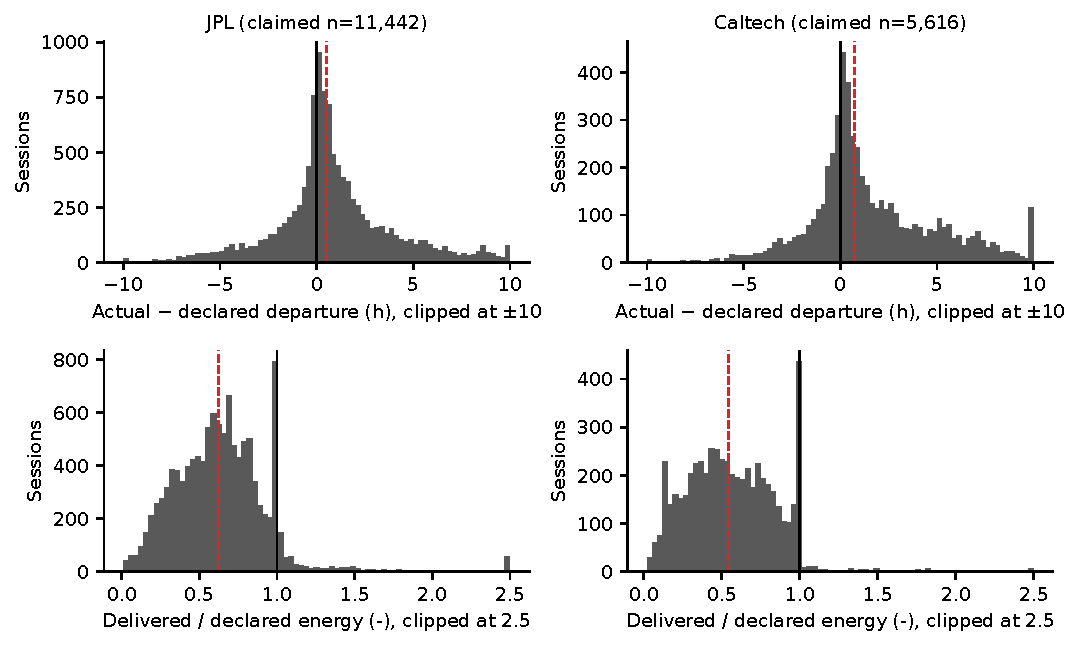
\includegraphics[width=0.7\textwidth]{figures/Fig3_declaration_errors.pdf}
\caption{Declaration errors of claimed sessions. Top: actual minus declared departure time. Bottom: delivered over declared energy. Dashed lines mark medians.}
\label{fig:errors}
\end{figure}

\subsection{Tariff}\label{sec:tariff}
We bill every policy under SCE Schedule TOU-EV-4 effective 1 March 2019 \cite{SCETOUEV4}, the tariff contemporaneous with the data, using the rate values encoded in the ACN research portal \cite{Lee2021ACNSim}. It combines time-of-use energy prices with a demand charge of 15.51\,USD per kW of monthly maximum demand. SCE's later commercial EV schedules carried a period without demand charges \cite{CPUCEVRates}, which would remove the problem studied here, so the demand-charge level is instead varied in the sensitivity analysis. General-service schedules for EV load on a shared building meter combine a facilities-related and a time-related demand charge \cite{SCETOUGS2}; our formulation includes both terms, and the time-related term is zero in the base case. In summer (June--September) weekday energy costs 0.05623\,USD/kWh at 23--08\,h, 0.0925\,USD/kWh at 08--12\,h and 18--23\,h, and 0.26668\,USD/kWh at 12--18\,h; the winter prices for the same periods are 0.06087, 0.07492 and 0.0869\,USD/kWh, and weekends are charged at the off-peak price (Table~S2 of the Supplementary Material). Holidays and customer charges are not modelled, and the EV load is assumed to be separately metered.


%======================================================================
\section{Methodology}\label{sec:method}
%======================================================================
Figure~\ref{fig:framework} summarises the framework.

\begin{figure}[!htbp]
\centering
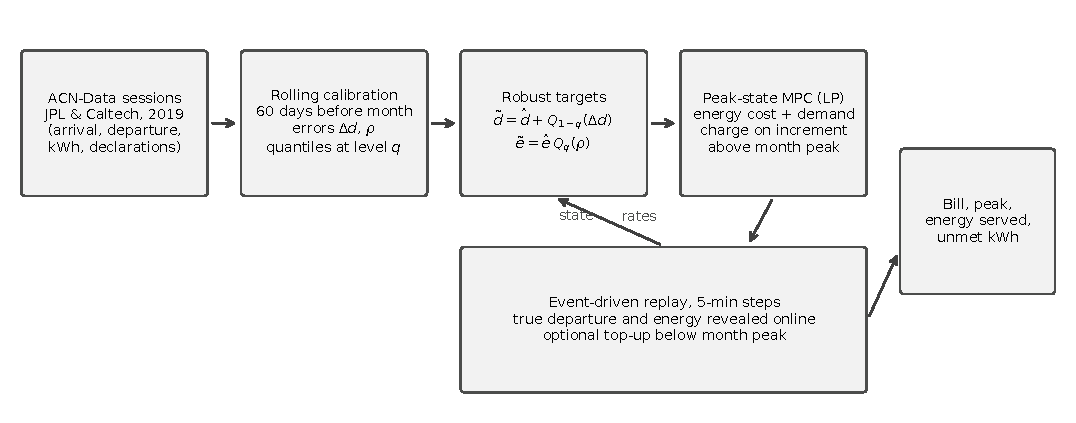
\includegraphics[width=0.7\textwidth]{figures/Fig1_framework.pdf}
\caption{Framework: rolling calibration of declaration errors, robust targets, peak-state MPC, and event-driven replay against realised sessions.}
\label{fig:framework}
\end{figure}

\subsection{Notation}
Time is discretised into periods $t\in\mathcal T=\{0,\dots,T-1\}$ of length $\Delta=5$\,min. Session $i\in\mathcal V$ arrives at $a_i$, departs at $d_i$ and accepts energy $e_i$ (kWh) at up to $\bar r_i$ (kW). At plug-in the controller observes a declaration $(\hat d_i,\hat e_i)$. The site capacity is $C$, energy prices are $c_t$ (USD/kWh), $\lambda^{F}$ is the facilities-related demand charge on the monthly maximum over all periods and $\lambda^{T}$ the time-related charge on the maximum over the set $\mathcal T^{\text{on}}$ of on-peak periods. The decision $r_{it}\ge0$ is the charging rate of session $i$ in period $t$.

\subsection{Hindsight benchmark}
With perfect knowledge of every $(a_i,d_i,e_i)$ in the month, the minimum bill solves the linear program
\begin{align}
\min_{r,s,P^F,P^T}\;& \sum_{t\in\mathcal T}\sum_{i\in\mathcal V} c_t\,\Delta\, r_{it} \;+\; \lambda^F P^F \;+\; \lambda^T P^T \;+\; M\sum_{i\in\mathcal V} s_i \label{eq:obj}\\
\text{s.t.}\;& \Delta\!\!\sum_{t=a_i}^{d_i-1}\! r_{it} + s_i \ge e_i,\qquad \Delta\!\!\sum_{t=a_i}^{d_i-1}\! r_{it}\le e_i, && i\in\mathcal V \label{eq:energy}\\
& 0\le r_{it}\le \bar r_i \;\;(a_i\le t<d_i),\qquad r_{it}=0\;\;\text{otherwise}, && i\in\mathcal V \label{eq:rate}\\
& \textstyle\sum_{i} r_{it}\le C, \qquad \sum_{i} r_{it}\le P^F, && t\in\mathcal T \label{eq:cap}\\
& \textstyle\sum_{i} r_{it}\le P^T, && t\in\mathcal T^{\text{on}} \label{eq:peakon}\\
& 0\le s_i\le e_i . \label{eq:slack}
\end{align}
The slack $s_i$ is undelivered energy penalised at $M$ (5\,USD/kWh in the base case; varied in Section~\ref{sec:sens}). The feasible set follows the ACN scheduling formulation \cite{Lee2019ACNData,Lee2021ACN}; the objective adds the demand charge as in \cite{Lee2020Pricing}.

\subsection{Peak-state receding-horizon control}
Online, at period $\tau$ the controller knows only the sessions present, their declarations, the energy already delivered $\delta_i(\tau)$, and the realised month-to-date peaks $\hat P^F(\tau)=\max_{t<\tau}\sum_i r_{it}$ and $\hat P^T(\tau)$ (the latter over on-peak periods). It solves \eqref{eq:obj}--\eqref{eq:slack} over the remaining horizon with three changes: (i) the window of session $i$ ends at its planning deadline rather than at its unknown departure, (ii) the energy target is the planning target minus $\delta_i(\tau)$, and (iii) the peak variables are bounded below by the realised peaks,
\begin{equation}
P^F\ge \hat P^F(\tau),\qquad P^T\ge \hat P^T(\tau). \label{eq:peakstate}
\end{equation}
Constraint~\eqref{eq:peakstate} makes the demand-charge term price only the increment $[P^F-\hat P^F(\tau)]^+$: capacity already paid for this month is free, which is the structural property of monthly demand charges that the controller must exploit. The LP is re-solved at every arrival, departure or completion event and at least every 15\,min; between solves the stored plan is applied. A vanishing tie-breaking term $\epsilon\sum_{i,t}(t-\tau)r_{it}$ favours earlier charging among cost-equivalent schedules, as in the deployed ACN \cite{Lee2019ACNData}. Following standard receding-horizon practice \cite{Mayne2014MPC}, only the first-period rates are implemented.

\subsection{Data-calibrated robust counterpart}\label{sec:robust}
Let $\mathcal U_i=[\underline{\Delta d},\overline{\Delta d}]\times[\underline\rho,\overline\rho]$ be a box of plausible declaration errors, so the true departure is $\hat d_i+\Delta d$ and the true energy $\rho\,\hat e_i$ for some $(\Delta d,\rho)\in\mathcal U_i$. A plan is robust for session $i$ if it delivers the required energy before departure for every realisation, i.e.
\begin{equation}
\Delta\!\!\sum_{t=\tau}^{\hat d_i+\Delta d-1}\! r_{it} \;\ge\; \rho\,\hat e_i-\delta_i(\tau)\qquad \forall(\Delta d,\rho)\in\mathcal U_i . \label{eq:robust}
\end{equation}
The left-hand side is non-decreasing in $\Delta d$ because $r_{it}\ge0$, and the right-hand side is increasing in $\rho$. The worst case is therefore attained at the corner $(\underline{\Delta d},\overline\rho)$ and \eqref{eq:robust} is equivalent to the single linear constraint
\begin{equation}
\Delta\!\!\sum_{t=\tau}^{\tilde d_i-1}\! r_{it} \ge \tilde e_i-\delta_i(\tau),\qquad \tilde d_i=\hat d_i+\underline{\Delta d},\quad \tilde e_i=\overline\rho\,\hat e_i . \label{eq:rc}
\end{equation}
This is Soyster's result for column-wise uncertainty \cite{Soyster1973} specialised to the EV constraint structure: the robust controller is the nominal controller with an earlier deadline and a scaled energy target, and it has exactly the same size. Because every constraint involves one session only, a cardinality budget across sessions \cite{Bertsimas2004Price} would not reduce conservatism for constraint-wise protection; conservatism is instead controlled by the size of the box.

\subsection{Rolling calibration}\label{sec:calib}
For a protection level $q\in(0,1)$ we set $\underline{\Delta d}=Q_{1-q}(\Delta d)$ and $\overline\rho=Q_q(\rho)$, the empirical quantiles of the errors observed in the 60 days before the test month, in the spirit of data-driven uncertainty sets \cite{Bertsimas2018DataDriven}. Claimed and unclaimed sessions are calibrated separately. For unclaimed sessions the declaration is a population prediction, the median stay and median energy of unclaimed training sessions with the same weekday flag and three-hour arrival bucket, and its errors are calibrated in the same way. The nominal controller corresponds to $(\underline{\Delta d},\overline\rho)=(0,1)$; $q=0.5$ gives a median-debiased controller, and $q=0.7$ and $0.9$ progressively more conservative ones. Energy delivered never exceeds the true $e_i$: when a vehicle is full its current drops to zero and the controller removes it, as a real system observes.

\subsection{Peak-state top-up}\label{sec:topup}
The robust counterpart can only move targets; it cannot deliver energy that the declarations do not ask for. The top-up rule exploits the same peak-state property as \eqref{eq:peakstate}, but after the LP has been solved. In each period, let $\bar P(\tau)=\min\{\hat P^F(\tau),C\}$, further limited by $\hat P^T(\tau)$ in on-peak periods when $\lambda^T>0$. Any headroom $\bar P(\tau)-\sum_i r_{i\tau}$ is then allocated to vehicles that still accept current, in order of declared departure, up to each vehicle's $\bar r_i$. By construction the top-up never raises a billed peak, so its only cost is the energy price of the additional kWh. We disclose that this rule was designed after, and because of, the diagnosis in Section~\ref{sec:res:diag} on the 2019 test months. To test it out of sample, we apply every policy unchanged to held-out 2021 sessions (Section~\ref{sec:res:heldout}) and under altered capacity, tariff, calibration and penalty settings (Section~\ref{sec:res:topuprob}). Both are simulation validations on recorded sessions, not a field deployment: drivers did not experience the top-up schedules, so behavioural responses to them are not captured.

\subsection{Grid-flexibility and solar-coincidence metrics}\label{sec:metrics}
Besides cost and service, we evaluate each realised monthly load profile $L_t$ with metrics of realised demand flexibility: peak reduction relative to uncontrolled charging, $\max_t L^{\text{unc}}_t-\max_t L_t$; the load factor $\bar L/\max_t L_t$ and its inverse, the peak-to-average ratio (PAR); the maximum change between consecutive 15-min averages (ramp); shifted energy, $\Delta\sum_t[L^{\text{unc}}_t-L_t]^+$; and the share of energy delivered in the weekday 12--18\,h on-peak block.
For the baseline, PV-unaware controllers, solar coincidence tests whether peak-state scheduling moves charging towards or away from solar hours. We build a clear-sky irradiance profile for each site with the Ineichen model in pvlib \cite{Holmgren2018pvlib,Anderson2023pvlib} and treat it as the output shape of a horizontal PV array. The array is sized so that its monthly energy equals the monthly EV demand ("energy-neutral"; a half-size array is a sensitivity). PV self-sufficiency is $\sum_t\min(L_t,PV_t)/\sum_t L_t$ and PV utilisation $\sum_t\min(L_t,PV_t)/\sum_t PV_t$.

\subsection{PV-aware peak-state control}\label{sec:pvaware}
To test whether the controller can exploit on-site generation rather than merely coincide with it, we add a behind-the-meter PV profile $PV_t$ (kW) and introduce the grid import $g_t\ge 0$ as a decision variable. The PV-aware controller solves \eqref{eq:obj}--\eqref{eq:slack} with the energy cost and both peaks applied to import instead of to EV load:
\begin{align}
g_t &\ge \textstyle\sum_i r_{it}-PV_t, \qquad g_t\le P^F\quad (t\in\mathcal T), \qquad g_t\le P^T\quad (t\in\mathcal T^{\text{on}}), \label{eq:pvaware}\\
&\text{with energy cost } \textstyle\sum_t c_t\,\Delta\, g_t \text{ replacing } \sum_{t,i} c_t\,\Delta\, r_{it} \text{ in \eqref{eq:obj}}. \nonumber
\end{align}
Surplus PV is assumed to be curtailed without export credit, so the controller is rewarded only for self-consumption. The top-up ceiling becomes $\min\{\hat P^F(\tau)+PV_\tau,\,C\}$, so top-up also absorbs surplus PV without raising the billed import peak. The PV profile is the energy-neutral clear-sky profile of Section~\ref{sec:metrics}. All policies, including PV-unaware ones, are billed on metered import in this scenario, so their costs are directly comparable.

\subsection{Transformer hosting limits}\label{sec:xfmr}
The site peak is only a proxy for distribution-network impact. To make the network dimension explicit, we represent the EV supply transformer as a hard import limit $\bar S$ and evaluate two hosting scenarios, in which the transformer rating is 50\% and 35\% of the six-month mean uncontrolled peak (148\,kW and 104\,kW at JPL; 52\,kW and 37\,kW at Caltech). They represent fleets on an existing transformer not sized for uncontrolled charging. Uncontrolled charging ignores the limit, and we report its maximum loading (per unit of rating), overload duration and overload energy. Controlled policies receive $\bar S$ as their capacity $C$; for them we report the energy service they can still deliver within the limit, which is the flexibility that is actually deliverable to the network operator.

\subsection{Tariff archetypes}\label{sec:archetypes}
To test transferability beyond the historical SCE schedule, we keep the TOU-EV-4 demand charge and evaluate two stylised archetypes: an \emph{evening-peak TOU}, with the on-peak block moved to 16--21\,h on weekdays as in recent tariffs of solar-rich systems, and a \emph{flat energy price} equal to the monthly time-weighted TOU-EV-4 mean, representing demand-charge tariffs without time-of-use energy prices. They are not actual tariffs; they isolate how the energy-price structure interacts with the demand charge.

%======================================================================
\section{Experimental design}\label{sec:design}
%======================================================================
\subsection{Policies}
We compare seven policy families on identical sessions: (1) \emph{Uncontrolled}, every vehicle charges at $\bar r_i$ from plug-in until full, without a capacity limit; (2) \emph{EDF}, earliest declared deadline first, and (3) \emph{LLF}, least declared laxity first, both allocating $\bar r_i$ in priority order up to $C$; (4) \emph{Nominal MPC}, the peak-state controller using declarations as given, which follows the design of \cite{Lee2020Pricing}; (5) \emph{Robust MPC}$(q)$ with $q\in\{0.5,0.7,0.9\}$; (6) \emph{MPC + top-up}, nominal and robust MPC ($q\in\{0.7,0.9\}$) with the rule of Section~\ref{sec:topup}; and (7) the \emph{hindsight optimum} of \eqref{eq:obj}--\eqref{eq:slack}, a lower bound on the penalised cost of any capacity-feasible policy. In the PV scenario, MPC + top-up and the hindsight optimum are also run in their PV-aware form (Section~\ref{sec:pvaware}).

\subsection{Replay and metrics}
Each test month (July--December 2019) is replayed at 5-min resolution. Sessions are assigned to the month of arrival, and the site capacities are 195\,kW (JPL) and 150\,kW (Caltech) \cite{Lee2019ACNData}. We report the monthly bill (energy plus demand charges on realised load), the monthly peak, the share of demanded energy served (demand being the energy each vehicle actually received in the recorded session, see below), the share of vehicles fully served (within 0.05\,kWh), and the bill gap to the hindsight optimum. LPs are solved with HiGHS \cite{Huangfu2018HiGHS} through SciPy and its Python interface \cite{Virtanen2020SciPy}. Because the ACN was itself a managed system, the recorded delivered energy may fall short of what some drivers would have taken without control; all service figures in this paper are therefore measured against historically delivered energy, not against unconstrained charging needs. Software integrity checks on synthetic data confirm that no controlled policy exceeds capacity, that delivered energy never exceeds demanded energy, and that the hindsight optimum lower-bounds the penalised cost of every controlled policy.

\subsection{Sensitivity analysis}\label{sec:sens}
For August and November 2019 we vary the demand charge (0 and twice the tariff value), the calibration window (30 and 90 days) and the shortfall penalty ($M=20$\,USD/kWh) for nominal MPC, robust MPC at $q=0.9$ and, where the objective changes, the hindsight optimum. The top-up rule is tested separately under these and further settings (Section~\ref{sec:res:topuprob}). Separately, a tariff-design sweep evaluates uncontrolled charging, MPC + top-up and the hindsight optimum for demand charges of 0, 5, 10, 15.51, 20 and 31.02\,USD/kW-month in the same two months. The PV-aware scenario covers all six test months; the transformer scenarios and tariff archetypes use August and November 2019.

%======================================================================
\section{Results}\label{sec:results}
%======================================================================
\subsection{Peak and bill reduction}
Tables~\ref{tab:main} and~\ref{tab:service} report six-month means with the range of monthly values, including the split of each bill into energy and demand charges. The demand charge is 69\% of the uncontrolled bill at both sites. At JPL uncontrolled charging exceeds the 195\,kW capacity (mean monthly peak 296\,kW), and EDF and LLF cut the bill by 23\% only by capping the peak at that limit; at Caltech the uncontrolled peak (105\,kW) never reaches the 150\,kW capacity, so EDF and LLF coincide with uncontrolled charging.

Nominal MPC reduces the mean monthly site peak from 296 to 140\,kW at JPL ($-53\%$) and from 105 to 52\,kW at Caltech ($-50\%$), a reduction of 156\,kW and 53\,kW of peak demand at the grid connection (monthly values in Fig.~S2). The mean monthly bill falls from 6,693 to 4,234\,USD at JPL ($-37\%$) and from 2,355 to 1,537\,USD at Caltech ($-35\%$). The weekday load profiles in Fig.~\ref{fig:profiles} show the mechanism: the controller flattens the morning arrival spike into a plateau and shifts energy away from the 12--18\,h summer on-peak window. The hindsight optimum shows how much is achievable with full information. With every session fully served it costs 3,913\,USD at JPL and 1,291\,USD at Caltech, with mean peaks of 110\,kW and 35\,kW.

\begin{table}[!htbp]
\centering
\caption{Monthly electricity cost by policy (July--December 2019).}
\label{tab:main}
\footnotesize
\setlength{\tabcolsep}{1.5pt}
\begin{tabular*}{\textwidth}{@{\extracolsep{\fill}}llrrrrr@{}}
\hline
Site & Policy & \makecell[c]{Bill\\(USD)} & \makecell[c]{Energy\\(USD)} & \makecell[c]{Demand\\(USD)} & \makecell[c]{Gap to\\opt. (\%)} & \makecell[c]{Penalised\\(USD)} \\
\hline
JPL & Uncontrolled & 6,693\,{\scriptsize(6,085--7,500)} & 2,103 & 4,589 & +74.0 & 6,693 \\
JPL & EDF & 5,171\,{\scriptsize(4,532--5,755)} & 2,146 & 3,024 & +33.7 & 5,289 \\
JPL & LLF & 5,147\,{\scriptsize(4,530--5,705)} & 2,123 & 3,024 & +33.2 & 5,156 \\
JPL & Nominal MPC & 4,234\,{\scriptsize(3,542--4,938)} & 2,066 & 2,168 & +8.9 & 8,468 \\
JPL & Robust MPC, $q$=0.5 & 3,079\,{\scriptsize(2,487--3,653)} & 1,763 & 1,317 & -21.1 & 27,951 \\
JPL & Robust MPC, $q$=0.7 & 3,705\,{\scriptsize(3,119--4,268)} & 1,975 & 1,730 & -4.7 & 15,625 \\
JPL & Robust MPC, $q$=0.9 & 4,586\,{\scriptsize(4,012--5,176)} & 2,052 & 2,534 & +18.6 & 8,531 \\
JPL & MPC + top-up & 4,376\,{\scriptsize(3,609--5,150)} & 2,208 & 2,168 & +12.4 & 4,610 \\
JPL & MPC + top-up, $q$=0.7 & 4,085\,{\scriptsize(3,290--4,876)} & 2,354 & 1,730 & +4.3 & 5,762 \\
JPL & MPC + top-up, $q$=0.9 & 4,681\,{\scriptsize(4,079--5,325)} & 2,157 & 2,524 & +20.9 & 4,754 \\
JPL & Hindsight opt. & 3,913\,{\scriptsize(3,086--4,682)} & 2,212 & 1,701 & +0.0 & 3,913 \\
\hline
Caltech & Uncontrolled & 2,355\,{\scriptsize(1,949--2,697)} & 729 & 1,627 & +86.3 & 2,355 \\
Caltech & EDF & 2,355\,{\scriptsize(1,949--2,697)} & 729 & 1,627 & +86.3 & 2,355 \\
Caltech & LLF & 2,355\,{\scriptsize(1,949--2,697)} & 729 & 1,627 & +86.3 & 2,355 \\
Caltech & Nominal MPC & 1,537\,{\scriptsize(1,092--1,795)} & 731 & 806 & +19.5 & 2,849 \\
Caltech & Robust MPC, $q$=0.5 & 1,000\,{\scriptsize(678--1,193)} & 550 & 450 & -22.6 & 10,883 \\
Caltech & Robust MPC, $q$=0.7 & 1,315\,{\scriptsize(954--1,628)} & 678 & 637 & +2.1 & 5,595 \\
Caltech & Robust MPC, $q$=0.9 & 1,515\,{\scriptsize(1,041--1,849)} & 716 & 799 & +17.3 & 3,731 \\
Caltech & MPC + top-up & 1,576\,{\scriptsize(1,102--1,869)} & 770 & 806 & +22.3 & 1,837 \\
Caltech & MPC + top-up, $q$=0.7 & 1,423\,{\scriptsize(989--1,814)} & 786 & 637 & +10.0 & 2,436 \\
Caltech & MPC + top-up, $q$=0.9 & 1,556\,{\scriptsize(1,063--1,895)} & 763 & 793 & +20.4 & 1,962 \\
Caltech & Hindsight opt. & 1,291\,{\scriptsize(895--1,607)} & 750 & 541 & +0.0 & 1,291 \\
\hline
\end{tabular*}
\par\smallskip\parbox{\textwidth}{\scriptsize Six-month means; the range of monthly values is shown in parentheses. Gap is the mean monthly bill gap to the hindsight optimum; Penalised adds 5\,USD per undelivered kWh.}
\end{table}


\begin{table}[!htbp]
\centering
\caption{Monthly peak demand and charging service by policy (July--December 2019).}
\label{tab:service}
\footnotesize
\setlength{\tabcolsep}{1.5pt}
\begin{tabular*}{\textwidth}{@{\extracolsep{\fill}}llrrr@{}}
\hline
Site & Policy & \makecell[c]{Peak\\(kW)} & \makecell[c]{Energy served\\(\%)} & \makecell[c]{EVs fully\\served (\%)} \\
\hline
JPL & Uncontrolled & 296\,{\scriptsize(284--313)} & 100.0\,{\scriptsize(100.0--100.0)} & 100.0\,{\scriptsize(100.0--100.0)} \\
JPL & EDF & 195\,{\scriptsize(195--195)} & 99.9\,{\scriptsize(99.9--99.9)} & 99.5\,{\scriptsize(99.3--99.7)} \\
JPL & LLF & 195\,{\scriptsize(195--195)} & 100.0\,{\scriptsize(100.0--100.0)} & 99.9\,{\scriptsize(99.8--100.0)} \\
JPL & Nominal MPC & 140\,{\scriptsize(128--154)} & 96.0\,{\scriptsize(94.9--97.3)} & 86.6\,{\scriptsize(84.1--89.1)} \\
JPL & Robust MPC, $q$=0.5 & 85\,{\scriptsize(78--91)} & 76.8\,{\scriptsize(75.3--78.1)} & 40.0\,{\scriptsize(37.7--43.3)} \\
JPL & Robust MPC, $q$=0.7 & 112\,{\scriptsize(103--116)} & 88.8\,{\scriptsize(87.9--90.6)} & 62.8\,{\scriptsize(60.1--65.2)} \\
JPL & Robust MPC, $q$=0.9 & 163\,{\scriptsize(151--173)} & 96.3\,{\scriptsize(95.4--97.3)} & 84.7\,{\scriptsize(81.0--87.0)} \\
JPL & MPC + top-up & 140\,{\scriptsize(128--154)} & 99.8\,{\scriptsize(99.7--99.9)} & 98.9\,{\scriptsize(98.5--99.7)} \\
JPL & MPC + top-up, $q$=0.7 & 112\,{\scriptsize(103--116)} & 98.4\,{\scriptsize(98.0--99.0)} & 94.0\,{\scriptsize(92.9--96.1)} \\
JPL & MPC + top-up, $q$=0.9 & 163\,{\scriptsize(150--173)} & 99.9\,{\scriptsize(99.8--100.0)} & 99.6\,{\scriptsize(99.1--99.9)} \\
JPL & Hindsight opt. & 110\,{\scriptsize(98--124)} & 100.0\,{\scriptsize(100.0--100.0)} & 100.0\,{\scriptsize(100.0--100.0)} \\
\hline
Caltech & Uncontrolled & 105\,{\scriptsize(89--121)} & 100.0\,{\scriptsize(100.0--100.0)} & 100.0\,{\scriptsize(100.0--100.0)} \\
Caltech & EDF & 105\,{\scriptsize(89--121)} & 100.0\,{\scriptsize(100.0--100.0)} & 100.0\,{\scriptsize(100.0--100.0)} \\
Caltech & LLF & 105\,{\scriptsize(89--121)} & 100.0\,{\scriptsize(100.0--100.0)} & 100.0\,{\scriptsize(100.0--100.0)} \\
Caltech & Nominal MPC & 52\,{\scriptsize(44--57)} & 96.3\,{\scriptsize(94.8--97.2)} & 87.6\,{\scriptsize(84.4--89.7)} \\
Caltech & Robust MPC, $q$=0.5 & 29\,{\scriptsize(24--33)} & 71.7\,{\scriptsize(69.3--76.0)} & 44.9\,{\scriptsize(40.6--49.6)} \\
Caltech & Robust MPC, $q$=0.7 & 41\,{\scriptsize(37--46)} & 87.9\,{\scriptsize(85.8--89.5)} & 65.3\,{\scriptsize(63.3--67.9)} \\
Caltech & Robust MPC, $q$=0.9 & 51\,{\scriptsize(42--55)} & 93.6\,{\scriptsize(91.8--95.5)} & 80.1\,{\scriptsize(77.8--82.2)} \\
Caltech & MPC + top-up & 52\,{\scriptsize(44--57)} & 99.2\,{\scriptsize(99.0--99.6)} & 96.0\,{\scriptsize(94.5--97.3)} \\
Caltech & MPC + top-up, $q$=0.7 & 41\,{\scriptsize(37--46)} & 97.1\,{\scriptsize(96.5--97.9)} & 90.5\,{\scriptsize(89.5--92.6)} \\
Caltech & MPC + top-up, $q$=0.9 & 51\,{\scriptsize(42--55)} & 98.8\,{\scriptsize(97.0--99.4)} & 95.9\,{\scriptsize(91.9--97.5)} \\
Caltech & Hindsight opt. & 35\,{\scriptsize(30--40)} & 100.0\,{\scriptsize(100.0--100.0)} & 100.0\,{\scriptsize(100.0--100.0)} \\
\hline
\end{tabular*}
\par\smallskip\parbox{\textwidth}{\scriptsize Six-month means with the range of monthly values in parentheses. A vehicle is fully served when its shortfall is at most 0.05\,kWh.}
\end{table}






\begin{figure}[!htbp]
\centering
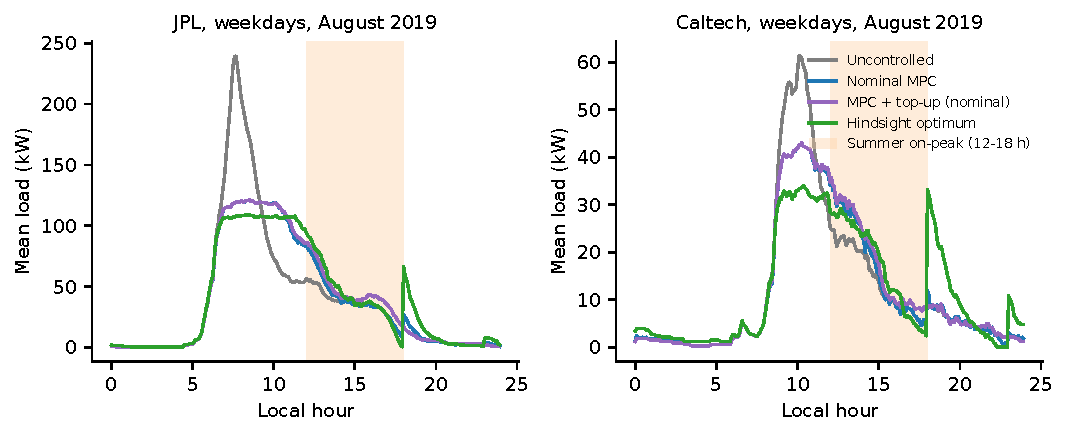
\includegraphics[width=0.7\textwidth]{figures/Fig4_load_profiles.pdf}
\caption{Mean weekday load profiles in August 2019. The shaded band is the TOU-EV-4 summer on-peak period.}
\label{fig:profiles}
\end{figure}

\subsection{Realised grid flexibility}\label{sec:res:flex}
Table~\ref{tab:flex} reports the grid-flexibility metrics of Section~\ref{sec:metrics}; normalised load-duration curves are shown in Fig.~S3 of the Supplementary Material.
\emph{Uncontrolled load is extremely peaky.} Its peak-to-average ratio is 10.2 (JPL) and 11.2 (Caltech): the site connection is sized for a load that occurs for a few hours on weekday mornings. \emph{Peak-state control roughly halves that ratio.} PAR falls to 4.8--5.0 (JPL) and 5.6--5.8 (Caltech), the load factor doubles, and the steepest 15-min ramp falls by 31\% (JPL) and 20\% (Caltech). This is achieved by moving 14--17\% (JPL) and 9--14\% (Caltech) of the monthly energy away from the time uncontrolled charging would have drawn it. \emph{Top-up does not erode the flexibility gain.} It leaves the peak unchanged and only raises the load factor further, because it fills existing headroom. \emph{Combining moderate robustness with top-up delivers most of the achievable flexibility.} At $q=0.7$ the peak reduction reaches 62\% (JPL) and 61\% (Caltech), close to the hindsight optimum (63\% and 67\%). The online controller also avoids the large ramps that the hindsight schedule produces at tariff-period boundaries at JPL (99\,kW per 15\,min, against 43\,kW). \emph{LLF delivers peak reduction only through the capacity cap.} It cuts the JPL peak by 34\% exactly to the 195\,kW limit and does nothing at Caltech, where capacity does not bind.
\begin{table}[!htbp]
\centering
\caption{Grid-flexibility metrics (July--December 2019).}
\label{tab:flex}
\footnotesize
\setlength{\tabcolsep}{1.5pt}
\begin{tabular*}{\textwidth}{@{\extracolsep{\fill}}llrrrrr@{}}
\hline
Site & Policy & \makecell[c]{Peak\\red. (\%)} & \makecell[c]{Load\\factor} & PAR & \makecell[c]{Max ramp\\(kW/15 min)} & \makecell[c]{Shifted\\(\%)} \\
\hline
JPL & Uncontrolled & 0.0\,{\scriptsize(0.0--0.0)} & 0.099 & 10.2\,{\scriptsize(8.8--10.8)} & 73.1 & 0.0 \\
JPL & LLF & 34.0\,{\scriptsize(31.3--37.7)} & 0.149 & 6.7\,{\scriptsize(5.9--7.1)} & 59.2 & 4.3 \\
JPL & Nominal MPC & 52.7\,{\scriptsize(45.6--56.1)} & 0.201 & 5.0\,{\scriptsize(4.0--5.6)} & 50.3 & 17.3 \\
JPL & Robust MPC, $q$=0.9 & 44.7\,{\scriptsize(40.8--51.5)} & 0.173 & 5.9\,{\scriptsize(4.7--6.5)} & 55.0 & 15.3 \\
JPL & MPC + top-up & 52.7\,{\scriptsize(45.6--56.1)} & 0.209 & 4.8\,{\scriptsize(3.9--5.4)} & 49.7 & 13.8 \\
JPL & MPC + top-up, $q$=0.7 & 62.3\,{\scriptsize(59.1--64.9)} & 0.258 & 3.9\,{\scriptsize(3.2--4.2)} & 42.9 & 20.1 \\
JPL & Hindsight opt. & 62.9\,{\scriptsize(56.2--67.6)} & 0.268 & 3.8\,{\scriptsize(3.0--4.3)} & 98.8 & 21.9 \\
\hline
Caltech & Uncontrolled & 0.0\,{\scriptsize(0.0--0.0)} & 0.091 & 11.2\,{\scriptsize(9.8--13.5)} & 34.3 & 0.0 \\
Caltech & LLF & 0.0\,{\scriptsize(0.0--0.0)} & 0.091 & 11.2\,{\scriptsize(9.8--13.5)} & 34.3 & 0.0 \\
Caltech & Nominal MPC & 49.9\,{\scriptsize(35.4--55.3)} & 0.176 & 5.8\,{\scriptsize(5.0--6.7)} & 27.4 & 13.7 \\
Caltech & Robust MPC, $q$=0.9 & 50.5\,{\scriptsize(42.0--58.0)} & 0.172 & 5.8\,{\scriptsize(5.3--6.3)} & 28.2 & 18.9 \\
Caltech & MPC + top-up & 49.9\,{\scriptsize(35.4--55.3)} & 0.181 & 5.6\,{\scriptsize(4.8--6.5)} & 27.2 & 9.3 \\
Caltech & MPC + top-up, $q$=0.7 & 60.6\,{\scriptsize(54.3--65.8)} & 0.224 & 4.5\,{\scriptsize(3.7--5.3)} & 23.4 & 15.8 \\
Caltech & Hindsight opt. & 66.7\,{\scriptsize(61.9--69.2)} & 0.272 & 3.7\,{\scriptsize(3.2--4.2)} & 34.9 & 22.1 \\
\hline
\end{tabular*}
\par\smallskip\parbox{\textwidth}{\scriptsize Means with monthly ranges in parentheses. Peak reduction and shifted energy are relative to uncontrolled charging; PAR is the peak-to-average ratio of the monthly load.}
\end{table}




\subsection{Coincidence with on-site solar}\label{sec:res:pv}
Flattening the morning spike moves charging towards midday, although the controllers receive no PV signal. With an energy-neutral clear-sky PV array, the share of EV energy coincident with PV rises from 46.7\% under uncontrolled charging to 53.4\% with MPC + top-up and 60.5\% at $q=0.7$ at JPL, and from 56.1\% to 59.7\% and 64.3\% at Caltech (Table~S3 and Fig.~S4 of the Supplementary Material; with a half-size array the gains have the same sign). The same shift has a cost under this tariff: the share of energy in the 12--18\,h on-peak block rises from 24.7\% to 28.3\% (JPL) and from 26.9\% to 33.9\% (Caltech), and the energy cost rises by about 5\%. The demand-charge and energy-price signals pull in opposite directions, and the demand charge wins because it is 69\% of the uncontrolled bill. Section~\ref{sec:res:pvaware} tests a PV-aware objective and Section~\ref{sec:res:arch} tariffs that remove this conflict.

\subsection{The service cost of acting on declarations}\label{sec:res:diag}
The bill reduction of nominal MPC is not free. It serves 96.0\% (JPL) and 96.3\% (Caltech) of the demanded energy, and only 86.6\% and 87.6\% of vehicles leave with their full energy. The hindsight optimum serves every vehicle at a lower bill, so the shortfall is caused by missing information, not by the tariff or the capacity limit. Valued at the base penalty of 5\,USD/kWh, the penalised cost of nominal MPC (8,468\,USD at JPL, 2,849\,USD at Caltech) is higher than that of LLF at JPL and of uncontrolled charging at Caltech.

Fig.~\ref{fig:unmet} decomposes the undelivered energy into its two causes. The first is vehicles whose declared energy was delivered but was below what they actually accepted: 45\% of the 5,080\,kWh left undelivered at JPL over the six months, and 31\% of 1,575\,kWh at Caltech. The second is vehicles that departed before their declared energy had been delivered (the remaining 55\% and 69\%). Both causes follow from the declaration errors in Fig.~\ref{fig:errors}. Most drivers over-request energy, but a minority under-request, and about a third leave earlier than declared.

\begin{figure}[!htbp]
\centering
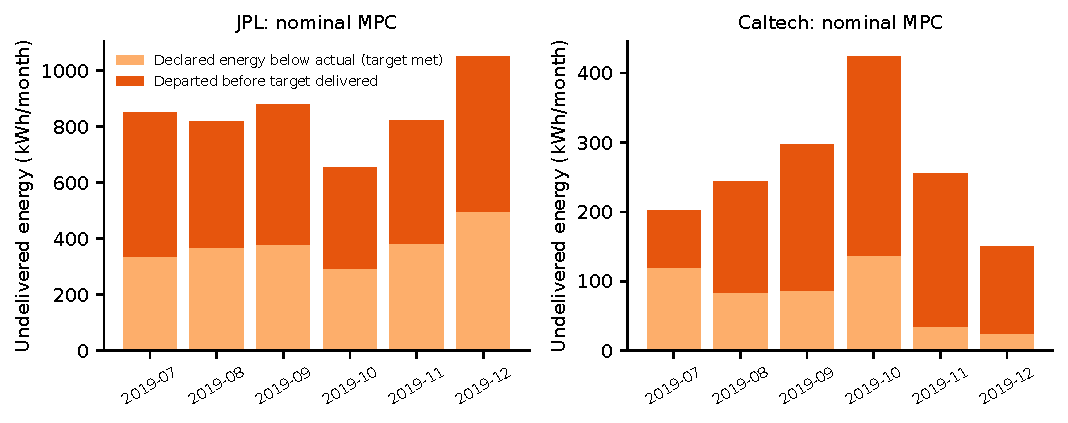
\includegraphics[width=0.7\textwidth]{figures/Fig10_unmet_decomposition.pdf}
\caption{Undelivered energy of nominal MPC by cause: declared energy below the energy actually accepted (target met), and departure before the declared energy was delivered.}
\label{fig:unmet}
\end{figure}

\subsection{Calibrated robustness does not close the gap}\label{sec:res:robust}
The calibrated sets are shown in Fig.~S5 of the Supplementary Material. At $q=0.5$ the controller moves deadlines 0.5--1\,h later and scales declared energy down to 0.52--0.65 of its declared value, because the median driver stays longer and receives less than declared. At $q=0.9$ deadlines move 1.3--2.8\,h earlier while the energy multiplier only returns to about 1.0. The upward bias of declared energy is so strong that even the 90th percentile of $\rho$ does not exceed one for claimed sessions.



The consequences are shown in Fig.~\ref{fig:frontier}. Robust MPC at $q=0.5$ and $0.7$ produces the lowest bills in the study, below the hindsight optimum at JPL for both levels and at Caltech for $q=0.5$. It does so by delivering only 72--89\% of the energy, so the saving is a service cut rather than better scheduling. At $q=0.9$ the energy served returns to the nominal level at JPL (96.3\%) but the earlier deadlines raise the peak to 163\,kW, increasing the bill by 8\% over nominal MPC. At Caltech, energy served at $q=0.9$ (93.6\%) remains below nominal. No protection level improves on nominal MPC in penalised cost at either site. The quantile box can shift and scale targets, but it cannot create energy targets for the minority of vehicles whose needs exceed their declarations, and protecting early leavers requires deadlines so early that the peak rises.

\begin{figure}[!htbp]
\centering
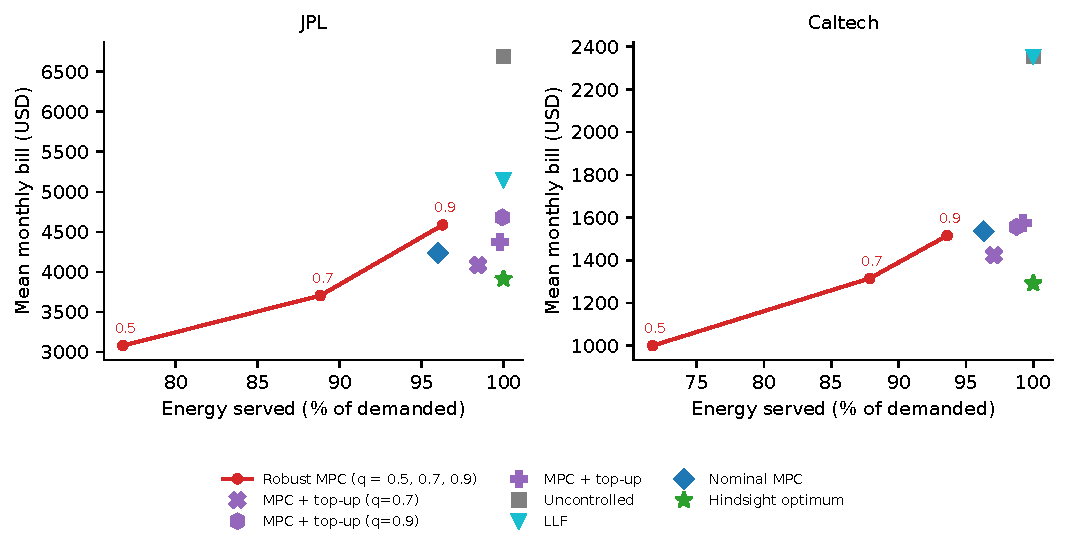
\includegraphics[width=0.7\textwidth]{figures/Fig5_price_of_robustness.pdf}
\caption{Bill against energy served (six-month means). Robust MPC traces a trade-off that stays inside the region reachable by the hindsight optimum; the top-up variants move close to full service.}
\label{fig:frontier}
\end{figure}

\subsection{Peak-state top-up}\label{sec:res:topup}
The top-up rule changes the picture (Table~\ref{tab:main}, Fig.~\ref{fig:frontier}). It is best understood as a more efficient use of electrical capacity: the site has already paid, through the demand charge, for a connection of $\hat P^F$ kilowatts this month, and top-up turns otherwise idle paid-for capacity into delivered EV energy. Applied to nominal MPC, it raises energy served to 99.8\% at JPL and 99.2\% at Caltech, and vehicles fully served to 98.9\% and 96.0\%. The monthly peak and demand charge stay exactly those of nominal MPC. The added cost is the energy price of the extra kWh: 142\,USD per month at JPL for about 800\,kWh, and 39\,USD per month at Caltech for about 210\,kWh, roughly 0.18--0.19\,USD/kWh. The bill remains 35\% (JPL) and 33\% (Caltech) below uncontrolled charging, and 15\% below LLF at JPL. The penalised cost falls to 4,610\,USD at JPL and 1,837\,USD at Caltech, the lowest of all online policies at both sites.

Combining top-up with robust targets gives a tunable operating point. At $q=0.7$ the lower targets keep the peak at 112\,kW (JPL) and 41\,kW (Caltech), and the top-up then serves 98.5\% and 97.1\% of energy. The JPL bill is 4,085\,USD, within 4.3\% of the hindsight optimum on average. At $q=0.9$ with top-up, service at JPL reaches 99.9\% (99.6\% of vehicles), but the higher peak costs 20.9\% over the optimum. Operators can therefore choose between a lower bill and fuller service with one parameter, provided top-up is present; without top-up, the same parameter only trades service for cost.

\subsection{Sensitivity}
Table~S4 of the Supplementary Material reports the sensitivity runs for August and November. Without a demand charge the controllers have no reason to flatten load, and the JPL peak rises to the 195\,kW capacity (Section~\ref{sec:res:tariff}). With twice the demand charge, nominal MPC still serves 96.1\% (JPL) and 95.2\% (Caltech) of energy, whereas robust MPC at $q=0.9$ serves only 91.2\% and 74.2\%, because its earlier deadlines can only be met by raising a peak that costs more than the shortfall penalty. With 30- or 90-day calibration windows, bills and energy served change by less than 1\%, so the negative result is not an artefact of the window length. Raising the shortfall penalty to 20\,USD/kWh leaves service at about 96\%: the shortfall follows from the targets the declarations set, which is why more information or top-up fixes it and re-weighting the objective does not.

\subsection{Tariff design determines whether flexibility is delivered}\label{sec:res:tariff}
Fig.~\ref{fig:tariff} shows how the demand-charge level changes what peak-state control delivers. The sweep uses August and November only (uncontrolled peaks 308 and 116\,kW).
\emph{Without a demand charge, no peak reduction is delivered.} At Caltech the controlled peak equals the uncontrolled peak (116\,kW in August and November). At JPL the only reduction (37\%) is the one the 195\,kW capacity limit imposes on every controlled policy. Without a demand charge, MPC + top-up cannot lower the bill: at JPL it is 1\% more expensive than uncontrolled charging because top-up then fills capacity regardless of price. \emph{A modest demand charge is enough to obtain almost all of the controller's peak reduction.} At 5\,USD/kW-month, about a third of the TOU-EV-4 value, the peak reduction is 55--56\%, essentially the same as at the tariff value (54--56\%) and at twice that value (56--60\%). Beyond this point the demand-charge level mainly scales the monetary saving: 21\% at 5\,USD/kW-month, 37\% at the tariff value and 45--48\% at twice that value. \emph{The online controller's peak saturates while the optimum's does not.} With perfect information the optimum keeps lowering the peak as the demand charge rises, to 68\% reduction at both sites. The online controller's peak is limited by the information available at the time of each decision rather than by the price.
The existence of a demand charge, rather than its exact level, therefore decides whether smart charging delivers local peak reduction. Tariff architecture is thus a precondition for realising the flexibility that controllers can technically provide.





\begin{figure}[!htbp]
\centering
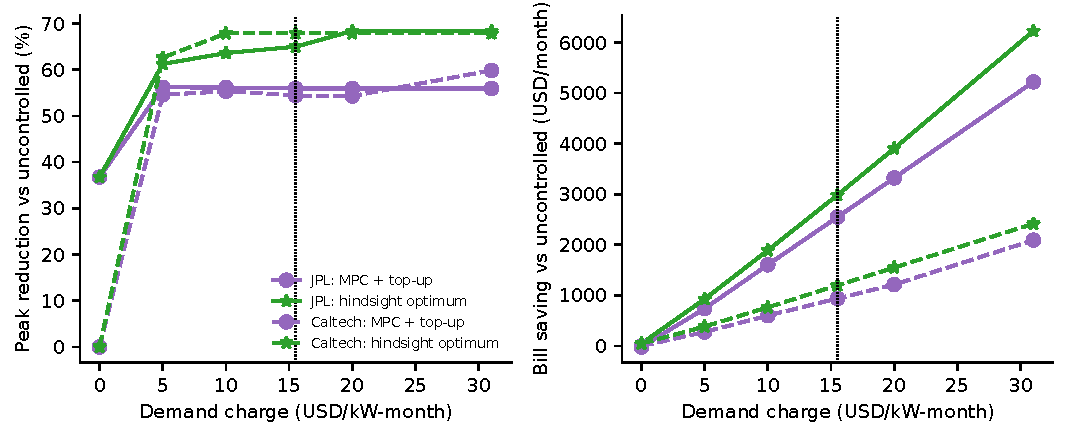
\includegraphics[width=0.7\textwidth]{figures/Fig13_tariff_design.pdf}
\caption{Tariff-design sweep (August and November 2019): peak reduction and monthly bill saving relative to uncontrolled charging as functions of the demand charge. The dotted line marks the TOU-EV-4 value.}
\label{fig:tariff}
\end{figure}

\subsection{Out-of-sample validation on held-out 2021 sessions}\label{sec:res:heldout}
Because top-up was designed after the 2019 diagnosis, we test all policies unchanged on the 2021 extract. Calibration uses the 60 days before each test month (May--June 2021), and the tests cover July and August 2021 (1,605 JPL and 836 Caltech sessions). It is a demanding test: volumes are lower after the pandemic and driver behaviour has shifted: the median claimed driver now leaves 0.4--0.5\,h (JPL) and 1.8--2.0\,h (Caltech) earlier than declared, instead of later, and the median delivered-to-declared energy ratio falls to 0.53--0.54 and 0.40--0.41. Table~\ref{tab:heldout} reports the results.
\emph{The service gap reappears, larger.} Nominal MPC cuts the bill by 30\% (JPL) and 43\% (Caltech) and the peak by 42\% and 53\%, but serves only 91.0\% and 83.7\% of the energy, with 81.7\% and 75.7\% of vehicles fully served. \emph{Top-up replicates.} MPC + top-up raises energy served to 98.6\% (JPL) and 97.1\% (Caltech) and vehicles fully served to 96.3\% and 95.0\%, with exactly the same peaks as nominal MPC. Bills remain 24\% and 34\% below uncontrolled charging. At JPL its penalised cost (3,580\,USD) is the lowest of all online policies and below LLF and uncontrolled charging (3,737\,USD). At Caltech it is the lowest online value but slightly above uncontrolled charging (1,327 against 1,261\,USD), because the remaining 2.9\% shortfall, valued at 5\,USD/kWh, outweighs the bill saving at this small site. \emph{Calibrated robustness fails more severely.} Under the behavioural shift, the $q=0.9$ deadline shifts move 5--8\,h earlier. The resulting targets can only be met by raising the peak, so the controller accepts shortfalls: energy served falls to 56\% (JPL) and 35\% (Caltech), and top-up recovers only part of it. At $q=0.7$ with top-up, JPL still reaches 97.3\% served, but Caltech only 84.2\%.
The held-out test thus confirms both central findings out of sample: top-up retains the peak and bill reductions with near-complete service, and quantile robustness calibrated on declarations is fragile once behaviour drifts.

\begin{table}[!htbp]
\centering
\caption{Out-of-sample validation on held-out 2021 sessions (means over July and August 2021).}
\label{tab:heldout}
\footnotesize
\setlength{\tabcolsep}{1.5pt}
\begin{tabular*}{\textwidth}{@{\extracolsep{\fill}}llrrrrrr@{}}
\hline
Site & Policy & \makecell[c]{Bill\\(USD)} & \makecell[c]{Saving vs\\unc. (\%)} & \makecell[c]{Peak\\(kW)} & \makecell[c]{Served\\(\%)} & \makecell[c]{EVs\\full (\%)} & \makecell[c]{Penalised\\(USD)} \\
\hline
JPL & Uncontrolled & 3,737 & +0.0 & 151.0 & 100.0 & 100.0 & 3,737 \\
JPL & LLF & 3,737 & +0.0 & 151.0 & 100.0 & 100.0 & 3,737 \\
JPL & Nominal MPC & 2,614 & +30.0 & 87.4 & 91.0 & 81.7 & 7,078 \\
JPL & Robust MPC, $q$=0.7 & 2,423 & +34.9 & 79.3 & 85.2 & 63.9 & 9,893 \\
JPL & Robust MPC, $q$=0.9 & 1,459 & +61.1 & 36.3 & 55.8 & 40.3 & 24,099 \\
JPL & MPC + top-up & 2,822 & +24.4 & 87.4 & 98.6 & 96.3 & 3,580 \\
JPL & MPC + top-up, $q$=0.7 & 2,705 & +27.4 & 79.2 & 97.3 & 92.7 & 4,167 \\
JPL & MPC + top-up, $q$=0.9 & 1,580 & +58.0 & 36.3 & 62.4 & 51.1 & 20,834 \\
JPL & Hindsight opt. & 2,468 & +34.5 & 63.7 & 100.0 & 100.0 & 2,468 \\
\hline
Caltech & Uncontrolled & 1,261 & +0.0 & 52.7 & 100.0 & 100.0 & 1,261 \\
Caltech & LLF & 1,261 & +0.0 & 52.7 & 100.0 & 100.0 & 1,261 \\
Caltech & Nominal MPC & 723 & +42.5 & 24.9 & 83.7 & 75.7 & 3,402 \\
Caltech & Robust MPC, $q$=0.7 & 521 & +58.2 & 13.6 & 68.9 & 54.9 & 5,786 \\
Caltech & Robust MPC, $q$=0.9 & 262 & +79.2 & 6.9 & 35.4 & 28.2 & 10,932 \\
Caltech & MPC + top-up & 827 & +34.1 & 24.9 & 97.1 & 95.0 & 1,327 \\
Caltech & MPC + top-up, $q$=0.7 & 601 & +51.8 & 13.3 & 84.2 & 80.7 & 3,328 \\
Caltech & MPC + top-up, $q$=0.9 & 349 & +72.4 & 6.9 & 52.3 & 47.4 & 8,223 \\
Caltech & Hindsight opt. & 776 & +38.5 & 22.1 & 99.9 & 99.3 & 798 \\
\hline
\end{tabular*}
\par\smallskip\parbox{\textwidth}{\scriptsize Calibration uses the 60 days before each test month. EDF coincides with LLF and is omitted.}
\end{table}


\subsection{Robustness of the top-up rule}\label{sec:res:topuprob}
Because the top-up rule was designed after the 2019 diagnosis, we also test it, unchanged, under conditions it was not designed for: a site capacity cut to 75\% and 50\% of its value, twice the demand charge, 30- and 90-day calibration windows, and a shortfall penalty of 20\,USD/kWh (four times the base value). Each scenario is run on August and November 2019 and on the held-out July and August 2021 (Table~S5 of the Supplementary Material).
The service gain persists in every scenario: top-up raises energy served from 94.1--96.5\% to 97.1--99.8\% in 2019 and from 83.0--91.5\% to 95.6--98.7\% in 2021, a gain of 2.4--3.7 and 7.2--13.5 percentage points. It never raises the peak: across all 56 scenario--site--month runs, the MPC + top-up peak equals the nominal MPC peak, except in one month where it is 1.8\,kW lower because energy delivered early reduced later needs. The weakest cases are those where capacity or cost binds. With JPL's capacity halved to 97.5\,kW, the limit binds below the nominal peak and top-up serves 97.1\% in 2019, with 90.9\% of vehicles fully served. With twice the demand charge, Caltech reaches 97.6\% (2019) and 95.6\% (2021), because the controller holds a lower peak and leaves less headroom to fill. These tests, like the held-out evaluation, are simulations on recorded sessions. They show that the rule's benefit does not depend on the particular settings under which it was devised; they do not show how drivers would respond to it in operation, which only a field trial can establish. Because service is measured against historically delivered energy, which the ACN's own controller may have truncated, we also raise every session's need to 1.1 and 1.25 times its recorded energy, capped at what its estimated maximum rate can deliver while plugged in, leaving declarations unchanged (Table~S6). Total demand then rises by 8--10\% and 18--23\%. Nominal MPC falls to 81--95\% served, whereas MPC + top-up still serves 96.0--99.5\%, never with a higher peak than nominal MPC, and with peak reductions of 43--61\%; the hindsight optimum serves at least 99.7\%. The larger the unrecorded demand, the larger the gain from top-up, because the extra energy is exactly what declarations do not request.


\subsection{PV-aware control: from coincidence to self-consumption}\label{sec:res:pvaware}
Table~\ref{tab:pv} reports the PV scenario of Section~\ref{sec:pvaware}. Its figures are scenario estimates under clear-sky irradiance with a horizontal, energy-neutral array, not verified performance under measured solar conditions. With an energy-neutral PV array behind the meter, uncontrolled charging still sets an import peak of 282\,kW at JPL and 79\,kW at Caltech, because the morning arrival spike precedes most of the solar output.
\emph{At JPL, PV awareness adds a large second layer of flexibility.} PV-unaware MPC + top-up lowers the import peak to 128\,kW. Making the controller PV-aware lowers it further to 73\,kW, 26\% of the uncontrolled value. The bill falls by another 32\% (from 2,777 to 1,878\,USD), PV self-sufficiency rises from 50.7\% to 58.0\%, and 99.2\% of energy is still served. With moderate robustness ($q=0.7$) the import peak reaches 46\,kW and self-sufficiency 64.4\%, close to the PV-aware optimum (43\,kW; 66.5\%), at 97.0\% energy served. \emph{At Caltech, PV awareness alone adds nothing.} The PV-aware and PV-unaware top-up controllers give almost the same import peak (26 and 25\,kW) and self-sufficiency (about 60\%), because Caltech's later arrivals already coincide with solar output. Only the robust variant moves further (16\,kW; 63.6\%), and the optimum shows that 72.7\% self-sufficiency would be attainable with perfect information.
The value of renewable-aware control is therefore site-specific. It is largest where arrivals precede solar output. As with the demand charge, the gap to the optimum is limited by the information drivers provide rather than by the solar resource.

\begin{table}[!htbp]
\centering
\caption{PV-aware control with an energy-neutral clear-sky PV array (means over July--December 2019; all policies billed on grid import).}
\label{tab:pv}
\footnotesize
\setlength{\tabcolsep}{1.5pt}
\begin{tabular*}{\textwidth}{@{\extracolsep{\fill}}llrrrrrr@{}}
\hline
Site & Policy & \makecell[c]{Bill\\(USD)} & \makecell[c]{Import\\peak (kW)} & \makecell[c]{Served\\(\%)} & \makecell[c]{EVs\\full (\%)} & \makecell[c]{PV self-\\suff. (\%)} & \makecell[c]{Penalised\\(USD)} \\
\hline
JPL & Uncontrolled & 5,190 & 281.9\,{\scriptsize(264--297)} & 100.0 & 100.0 & 46.7 & 5,190 \\
JPL & Top-up, PV-unaware & 2,777 & 127.6\,{\scriptsize(121--135)} & 99.9 & 99.5 & 50.7 & 2,876 \\
JPL & PV-aware top-up & 1,878 & 73.3\,{\scriptsize(57--94)} & 99.2 & 97.3 & 58.0 & 2,692 \\
JPL & PV-aware, $q$=0.7 & 1,447 & 46.2\,{\scriptsize(34--57)} & 97.0 & 91.2 & 64.4 & 4,626 \\
JPL & PV-aware opt. & 1,311 & 43.3\,{\scriptsize(38--47)} & 100.0 & 99.9 & 66.5 & 1,323 \\
\hline
Caltech & Uncontrolled & 1,487 & 79.3\,{\scriptsize(65--91)} & 100.0 & 100.0 & 56.1 & 1,487 \\
Caltech & Top-up, PV-unaware & 642 & 25.0\,{\scriptsize(19--31)} & 99.2 & 97.1 & 60.5 & 922 \\
Caltech & PV-aware top-up & 666 & 26.2\,{\scriptsize(21--35)} & 99.3 & 96.8 & 60.2 & 921 \\
Caltech & PV-aware, $q$=0.7 & 492 & 16.3\,{\scriptsize(15--21)} & 97.4 & 91.9 & 63.6 & 1,401 \\
Caltech & PV-aware opt. & 401 & 15.5\,{\scriptsize(12--21)} & 100.0 & 99.9 & 72.7 & 407 \\
\hline
\end{tabular*}
\par\smallskip\parbox{\textwidth}{\scriptsize Monthly range of the import peak below the mean. PV self-sufficiency is the share of delivered EV energy supplied by PV. Surplus PV is curtailed without export credit.}
\end{table}


\subsection{Transformer hosting limits: deliverable flexibility}\label{sec:res:xfmr}
Table~\ref{tab:xfmr} reports the transformer scenarios of Section~\ref{sec:xfmr}.
\emph{Uncontrolled charging overloads.} On a transformer rated at 50\% of its uncontrolled peak, uncontrolled charging reaches 2.1 (JPL) and 2.2 (Caltech) times the rating, for 38 and 32 hours per month. At a 35\% rating the loading reaches about 3 per unit for 54--57 hours per month, with 4,427\,kWh (JPL) and 1,141\,kWh (Caltech) of monthly energy above the rating. \emph{Within a 50\% rating, controlled charging delivers almost full service.} MPC + top-up stays at 0.92 (JPL) and 0.98 (Caltech) of the rating while serving 99.8\% and 99.0\% of energy, so its demand-charge-driven peak reduction already satisfies the network limit with headroom. \emph{At a 35\% rating, the limit binds for every online policy.} MPC + top-up then serves 98.4\% (JPL) and 96.6\% (Caltech) of energy, and LLF serves 98.3\% and 97.2\%. The hindsight optimum still serves 100\% and 99.7\% within the same rating. The limit is therefore physically compatible with full service; online controllers fall short because they lack information, not capacity. Under a tight network limit the simple LLF rule is as good as MPC on service, because the binding constraint is capacity rather than cost.
For a distribution operator, these results translate site-level control into a deliverable quantity. A workplace fleet that would load its transformer to two or three times its rating can be held within the rating, with only 0--3\% of energy unserved, by controllers that need nothing beyond plug-in events and meter readings. These are statements about a static import limit at the connection point. They show that the required energy fits under the rating, not that the transformer stays within its thermal limits, that feeder voltages remain in range or that phases stay balanced; Section~\ref{sec:discussion} returns to these limitations.

\begin{table}[!htbp]
\centering
\caption{Transformer hosting scenarios (means over August and November 2019).}
\label{tab:xfmr}
\footnotesize
\setlength{\tabcolsep}{1.5pt}
\begin{tabular*}{\textwidth}{@{\extracolsep{\fill}}lllrrrrr@{}}
\hline
Site & \makecell[c]{Rating\\kW (\%)} & Policy & \makecell[c]{Max loading\\(p.u.)} & \makecell[c]{Overload\\(h/mo)} & \makecell[c]{Overload\\(kWh/mo)} & \makecell[c]{Served\\(\%)} & \makecell[c]{EVs\\full (\%)} \\
\hline
JPL & 148 (50\%) & Uncontrolled & 2.08 & 37.8 & 2,342 & 100.0 & 100.0 \\
JPL & 148 (50\%) & LLF & 1.00 & 0.0 & 0 & 99.9 & 99.4 \\
JPL & 148 (50\%) & Top-up & 0.92 & 0.0 & 0 & 99.8 & 98.7 \\
JPL & 148 (50\%) & Top-up, $q$=0.7 & 0.74 & 0.0 & 0 & 98.6 & 94.3 \\
JPL & 148 (50\%) & Hindsight opt. & 0.73 & 0.0 & 0 & 100.0 & 100.0 \\
JPL & 104 (35\%) & Uncontrolled & 2.98 & 57.2 & 4,427 & 100.0 & 100.0 \\
JPL & 104 (35\%) & LLF & 1.00 & 0.0 & 0 & 98.3 & 95.4 \\
JPL & 104 (35\%) & Top-up & 1.00 & 0.0 & 0 & 98.4 & 93.8 \\
JPL & 104 (35\%) & Top-up, $q$=0.7 & 1.00 & 0.0 & 0 & 97.9 & 91.9 \\
JPL & 104 (35\%) & Hindsight opt. & 0.98 & 0.0 & 0 & 100.0 & 100.0 \\
\hline
Caltech & 52 (50\%) & Uncontrolled & 2.21 & 31.7 & 498 & 100.0 & 100.0 \\
Caltech & 52 (50\%) & LLF & 1.00 & 0.0 & 0 & 99.7 & 98.3 \\
Caltech & 52 (50\%) & Top-up & 0.98 & 0.0 & 0 & 99.0 & 95.4 \\
Caltech & 52 (50\%) & Top-up, $q$=0.7 & 0.81 & 0.0 & 0 & 96.7 & 89.8 \\
Caltech & 52 (50\%) & Hindsight opt. & 0.71 & 0.0 & 0 & 100.0 & 100.0 \\
Caltech & 37 (35\%) & Uncontrolled & 3.16 & 54.2 & 1,141 & 100.0 & 100.0 \\
Caltech & 37 (35\%) & LLF & 1.00 & 0.0 & 0 & 97.2 & 92.6 \\
Caltech & 37 (35\%) & Top-up & 1.00 & 0.0 & 0 & 96.6 & 90.1 \\
Caltech & 37 (35\%) & Top-up, $q$=0.7 & 1.00 & 0.0 & 0 & 95.5 & 87.9 \\
Caltech & 37 (35\%) & Hindsight opt. & 0.96 & 0.0 & 0 & 99.7 & 99.7 \\
\hline
\end{tabular*}
\par\smallskip\parbox{\textwidth}{\scriptsize Ratings are 50\% and 35\% of the six-month mean uncontrolled peak. Controlled policies treat the rating as a hard limit; uncontrolled charging does not.}
\end{table}




\subsection{Tariff archetypes}\label{sec:res:arch}
Under both stylised archetypes, which keep the demand charge (Table~S7 of the Supplementary Material), MPC + top-up reduces the peak by the same 56\% (JPL) and 54\% (Caltech) as under TOU-EV-4, with 99.8\% and 99.0\% of energy served: the demand charge, not the energy-price structure, drives peak reduction. The energy-price conflict disappears. Flattening raises the energy cost by 6.1\% (JPL) and 5.4\% (Caltech) under TOU-EV-4, but by only 2.6\% and $-0.7$\% under the evening-peak archetype and by $-0.2$\% and $-0.9$\% under a flat price, so the total bill saving rises from 37\% to 40--41\%. Tariffs that combine a demand charge with an evening peak or a flat energy price, as is common outside California, therefore reward both local peak reduction and midday solar absorption.

%======================================================================
\section{Discussion}\label{sec:discussion}
%======================================================================
\subsection{From technical to grid-usable flexibility}
The technical flexibility of workplace charging, bounded by parking duration and connected capacity, differs from the grid-usable flexibility that a controller can deliver while keeping drivers served and that a network operator can rely on. This requires evaluating charging service, operator cost and grid flexibility at the connection point jointly. Uncontrolled charging maximises service and minimises flexibility; robust MPC at low $q$ looks best on cost and peak alone precisely because it withholds energy, so assessments that report only one or two dimensions can rank policies wrongly. Service is measured here against the energy each vehicle received in 2019 under the ACN's own control, so a figure such as 99\% served means that the controllers reproduce the recorded energy deliveries, not that they meet every driver's unconstrained need; where the recorded deliveries were themselves truncated, true service would be lower for all policies alike. MPC + top-up is the only online policy that is close to the frontier on all three at once, and combining it with moderate robustness moves further along the flexibility axis at a small service cost.

\subsection{Information quality, not optimisation, limits realisable flexibility}
The negative result on calibrated robustness is an empirical energy-management finding, not a failure of the optimisation method: better mathematical protection cannot compensate for structurally poor information. Declared energy is an upper bound for most drivers and a lower bound for a few, and declared departure is late for about a third. Constraint-wise robust counterparts over boxes, whether built from quantiles as here or from more elaborate data-driven sets \cite{Bertsimas2018DataDriven,Esfahani2018Wasserstein}, can shift and scale targets but cannot add energy that no target requests, and they pay for early-leaver protection with higher peaks. What works is recourse to realised information: the observation that a vehicle is still drawing current, used by top-up. This is consistent with the caution against over-conservative robust solutions \cite{Bertsimas2004Price,Gorissen2015Guide}. It also suggests that per-driver prediction \cite{Lee2019ACNData,Wang2016Predictive,Kreft2024Predictability} and incentives for accurate declarations are the most promising levers for realising more of the flexibility that parking durations imply.

\subsection{Implications for energy-system actors}
\emph{Charging-site operators} gain roughly a third of the electricity bill and half of the site peak from demand-charge-aware control; greedy capacity-constrained rules capture peak reduction only where capacity binds. Headroom below the month's realised peak should be filled with top-up, which costs only the energy price, and energy served should always be reported alongside savings.
\emph{Aggregators and utilities} can treat the realised month-to-date peak $\hat P^F(\tau)$, set early in the billing month and then defended, as a verifiable firm-capacity limit offered to a distribution operator, aggregator or virtual power plant; the formulation extends to this by replacing the site peak with a contracted import limit or network signal. A controlled workplace fleet can be expected to deliver about half of its uncontrolled peak as firm reduction, enough to keep a half-rated transformer within its rating; in the clear-sky PV scenario, PV-aware control at a site like JPL lowers the import peak to about a quarter. Deeper reductions, up to the 63--68\% achieved in hindsight, need better information than declarations.
\emph{Tariff designers} should note that the presence of a demand charge, not its level, decides whether local peak reduction is delivered. Commercial EV rates that suspend demand charges \cite{CPUCEVRates} remove the incentive to flatten workplace load, whereas a small demand charge, or an equivalent subscription or import-limit product, unlocks it. Moving the on-peak energy window to the evening, or using a flat energy price, removes the conflict with midday charging.

\subsection{Deployment, network constraints and generalisability}
In real time, the controller needs plug-in events, declarations where available, a per-port signal showing whether a vehicle still draws current, the site meter reading and the tariff, all available in networked systems of the ACN type \cite{Lee2021ACN}. Each re-solve is a sparse LP that grows linearly with the connected vehicles and the horizon: mean solve times were 0.013\,s for JPL's 52 ports and 0.005\,s at Caltech on one core, and the monthly hindsight LP took 8.1\,s and 2.3\,s. Sites with hundreds of ports remain well within minute-scale control loops; top-up is a sorting step, and calibration needs only a rolling store of past sessions.

The transformer analysis is a static import limit. It does not model transformer thermal dynamics or ageing, feeder voltage, three-phase imbalance or power flow, all present in real installations \cite{Lee2021ACN,Lee2021ACNSim} and distribution networks \cite{ClementNyns2010,deHoog2015Network,Gong2012Transformer}. The peak-state structure is compatible with richer models: per-phase or per-transformer constraints can be added to the LP \cite{Lee2021ACN,deHoog2015Network}, transformer or feeder peaks can be tracked as additional peak states, and top-up then fills headroom below the tightest limit.

Three elements of the findings are structural and should transfer: the monthly peak-state logic, under which capacity paid for early in the month is free thereafter; the gap between declared and realised behaviour, documented in other datasets \cite{Kreft2024Predictability,Flammini2019Stats}; and the re-use of paid-for capacity through top-up. The TOU-EV-4 price windows, the commuting patterns of two southern Californian campuses, Level-2 charger power, site capacities and the 2019 period are context-specific, so the magnitudes reported here should be re-estimated elsewhere. The ordering of policies and the mechanism behind the robustness failure are expected to hold wherever declarations are biased and wide, as the held-out 2021 test and the tariff archetypes indicate.

\subsection{Limitations}
Vehicles are ideal loads that accept energy at up to $\bar r_i$ until full, without battery tapering, and $\bar r_i$ is estimated because the extract lacks the done-charging time. The energy delivered by the ACN is used as each vehicle's demand and may have been truncated by the controller in place at the time, so service figures measure delivery relative to historical charging, not necessarily drivers' actual needs; the higher-demand sensitivity (Section~\ref{sec:res:topuprob}) bounds, but does not remove, this uncertainty. The PV scenarios use clear-sky irradiance and a horizontal array, because measured irradiance for the sites was not accessible to us; they overstate solar output on cloudy days, and surplus PV is curtailed without export credit. Transformer limits are static, holidays and customer charges are omitted, and the study covers two sites, six test months and a two-month held-out period. The top-up rule was designed after the 2019 diagnosis and validated in simulation on two held-out 2021 months and under altered capacity, tariff, calibration and penalty settings; it has not been tested in a field deployment, where drivers might respond to the fuller service it offers.

%======================================================================
\section{Conclusions}\label{sec:conclusion}
%======================================================================
The flexibility of workplace EV charging is not determined only by how long cars are parked or how much charging capacity is connected. On 13,623 real sessions from two California workplaces, peak-state control that prices only increments above the month-to-date peak roughly halved the site peak (from 296 to 140\,kW and from 105 to 52\,kW). Acting on driver declarations, however, left about one vehicle in eight short of its energy, and robust counterparts calibrated to empirical declaration errors did not close this gap. Re-using capacity already billed in the month restored service to above 99\% of the historically delivered energy without a new peak; on held-out 2021 sessions, and under altered capacity, tariff and calibration settings, it again raised service to 96--99\% without raising the peak. These are simulation results on recorded sessions, not field results.

The same controllers held a transformer rated at half the uncontrolled peak within its rating with near-complete service, where uncontrolled charging overloaded it by a factor of two. In a clear-sky PV scenario, where arrivals precede solar output, PV-aware control lowered the import peak to about a quarter of its uncontrolled value. The presence of a demand charge, not its level or the energy-price structure, decided whether any peak reduction was delivered.

Information quality and tariff design therefore jointly determine how much of the technical flexibility of workplace charging can be realised without degrading mobility service. Future work should test the controllers in the field, over longer periods and at other sites; replace population-level uncertainty sets with per-driver predictions and declaration incentives; add transformer thermal, voltage and three-phase models as further peak states; and test the realised peak as a contracted flexibility product for aggregators and virtual power plants.


\section*{CRediT authorship contribution statement}
\textbf{Mansour Almuwallad:} Conceptualization, Methodology, Software, Data curation, Formal analysis, Investigation, Validation, Visualization, Writing -- original draft, Writing -- review and editing.

\section*{Declaration of competing interest}
The author declares no known competing financial interests or personal relationships that could have appeared to influence the work reported in this paper.

\section*{Funding}
This research did not receive any specific grant from funding agencies in the public, commercial, or not-for-profit sectors.

\section*{Data availability}
The session data analysed in this study are publicly available: ACN-Data \cite{Lee2019ACNData,ACNDataset}, in the extracts for May--December 2019 and May--August 2021 redistributed with SustainGym v0.1.7 under CC-BY-4.0 \cite{Yeh2023SustainGym}. Tariff values are those of SCE TOU-EV-4 as encoded in acnportal v0.3.3 \cite{SCETOUEV4}. All code, the session extracts with checksums, every per-month result, the replayed load profiles and the sources of all tables and figures are openly available in a public GitHub repository \cite{ThisStudyRepo}, released under the MIT licence (the ACN-Data extracts in it remain under CC-BY-4.0):\\ {\small\url{https://github.com/drmansouralmuwallad-png/workplace-ev-flexibility}}.\\ The repository README lists the commands that reproduce every result in this paper.

\section*{Declaration of generative AI and AI-assisted technologies in the manuscript preparation process}
During the preparation of this work the author used Claude (Anthropic) to assist with code development, literature retrieval and drafting. After using this tool, the author reviewed and edited the content as needed and takes full responsibility for the content of the published article.

\section*{Supplementary material}
Supplementary material (Tables S1--S7 and Figs.~S1--S5) is provided with this article.


\bibliographystyle{elsarticle-num}
\bibliography{references}
\end{document}
